\documentclass[11pt]{article}
\usepackage{indentfirst}
\usepackage{listings}
\usepackage{graphicx}
\usepackage{hyperref}
\usepackage{float}

\begin{document}
\title{\vspace{-5cm}A multi-resolution sinusoidal model}
\date{February 2020}
\author{Tomás Bilal Iaquinta}

\maketitle
\hrulefill
\pagenumbering{arabic}

\section{Sound selection}

The sounds selected for the assignment are:

\begin{itemize}
	\item \href{https://freesound.org/people/xserra/sounds/217543/}{Chinese Orchestra}.
	\item \href{https://freesound.org/people/Ionicsmusic/sounds/193772/}{Drum \& Bass}.
\end{itemize}

The first audio file is the same one used throughout the course (\textit{orchestra.wav}), which represent a short sample of 6 seconds of a Chinese orchestra, where it i possible to hear a multiplicity of instruments. It was chosen for this reason since it represents a complex function where there are different pitched sound sources. \vspace{8pt}

The second audio consist only of a drum kit and an electric bass, playing simultaneously for 5 seconds. These two elements represent a signal with more transients (characteristics of percussive instruments), and a melodic signal where a pitch and harmonics are easily perceived.

\section{Procedure}
\subsection{Chinese Orchestra}

Using the software \textit{Sonic Visualizer} we can plot the spectogram of the sound to see where the tonal information is located and the overall characteristic of its spectrum through the length of the audio. 

\begin{figure}[h]
  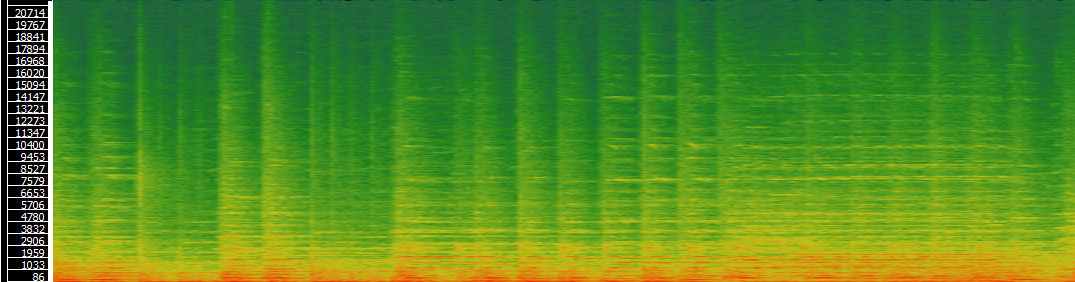
\includegraphics[width=\linewidth]{orch.png}
  \caption{Spectogram of the Chinese Orchestra sound.}
  \label{fig:orch}
\end{figure}

In Figure \ref{fig:orch} it is possible to see a high tonal energy  Clear horizontal lines corresponding to the harmonics, are seen until around 5 kHz, having low energy in higher frequencies. After changing the plot scale of the above graph to logarithmic, it is estimated that pitch (or what can be high frequency harmonics) from different instruments are located up to 1 kHz. This limits will represent where the analysis window changes in the generated function. The longest window will be applied for the \textit{'pitch zone'}, and with a narrow main-lobe.

\subsection{Drum \& Bass}

The first step is to convert the Drum \& Bass snippet to one-channel (mono) audio file, which is done by using \textit{Audacity}. Similar to what was done for the orchestra, the spectrogram is analyzed to select the frequency limits for the generated multi-resolution sinusoidal model applied. 

\begin{figure}[h]
  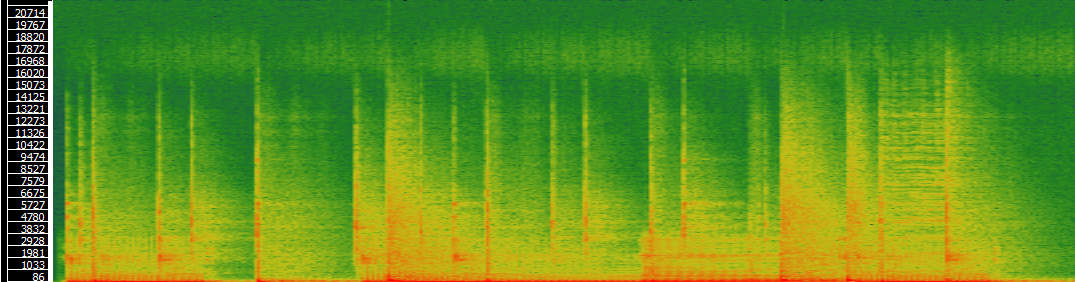
\includegraphics[width=\linewidth]{dbv.png}
  \caption{Spectrogram of the Drum \& Bass snipet.}
  \label{fig:dbv}
\end{figure}

Figure \ref{fig:dbv} shows a much different behaviour. Harmonic frequency lines appear much more separated (since they come from only one source), and more clear vertical lines are appreciated, which represent transients. Since lower harmonics seem to have more relative energy than the previous sound, the first limit will be higher in frequency. In one of the last notes it is possible to see clear harmonics up to 13 kHz which will be our second frequency limit.

\section{Software results}

A new function called \texttt{sineModel\_multi()} is created for the purpose of this assignment, being based on the existing \texttt{sineModel()} function. Please see the attached code for obtaining the same output. Next, we analyze with the following parameters:

\begin{itemize}
	\item{\textbf{Windows:} \texttt{'hamming', $(2^{12})$-1}, \texttt{'blackman', $(2^{10})$-1}, \texttt{'blackman', $(2^8)$-1}} 
	\item{\textbf{Frequency limits:} Orchestra: [990 Hz 5.6 kHz], D\&B: [2.5 kHz, 13 kHz]}
\end{itemize}

The windows will be getting smaller for upper frequencies, where there is not so much harmonic information. And in the frequencies from 0 Hz to the  the first limit, a \texttt{Hamming} window is applied with a long number of samples, being the objective to get accurately the pitch and first harmonics of the instruments.

\begin{figure}[H]
  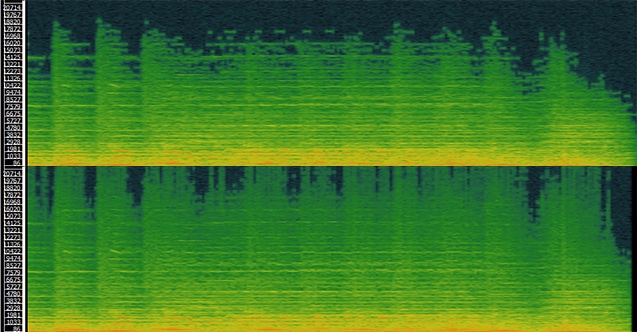
\includegraphics[width=\linewidth]{orch_out.jpg}
  \caption{Spectrogram comparison for the Chinese Orchestra between the regular Sinusoidal model (above), and the multi-resoultion one created (below).}
  \label{fig:orch_out}
\end{figure}

\begin{figure}[h]
  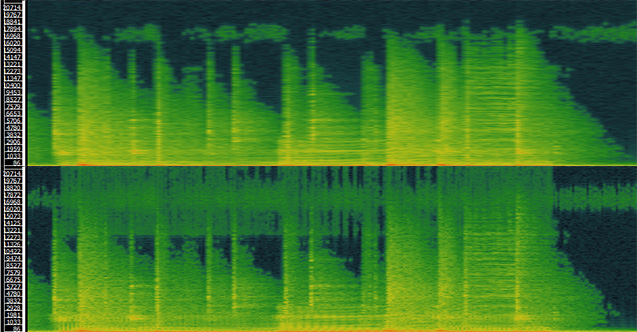
\includegraphics[width=\linewidth]{dbv_out.jpg}
  \caption{Spectrogram comparison for the Drum \& Bass snippet between the regular Sinusoidal model (above), and the multi-resoultion one created (below).}
  \label{fig:dbv_out}
\end{figure}

In Figure \ref{fig:orch_out} and Figure \ref{fig:dbv_out}, we can see a spectrogram comparison from the analysis as specified (above on each pictures), and the equivalent \texttt{sineModel()} output using the middle window (the one used in between both frequency limits.

\section{Conclusions}

Having heard both representations and seeing the spectrograms, it is clear that using a multi-resolution model we get a best representation. Having the advantages of a long window to capture the pitch and first harmonics, while also capturing more energy in the higher frequency spectrum (which can be seen in the plots), by using a shorter window. This way prioritizing with the window time over frequency resolution in this part of the spectrum.

Overall the model has a better performance but has a considerable higher computational cost, which has to be considered when analyzing long audio files. A better representation yet may be achieved playing some more with the input to the created function, feel free to try it !.\vspace{8pt}

If we were to try this implementation with the \texttt{HPR} or \texttt{HPS} model, one thing to consider is that we may have problems when the pitch of the instrument changes. Since we change the window at a certain frequency bin, the pitch may pass this region and its representation will change. One possibility would be to keep changing the frequency limits along with the frames of the sound. On the other hand, since we have the advantage of using different windows the computation of the $f_0$ could be easier since we can choose in the lower frequency band, for example, a \texttt{Blackman} window if we need side-lobe attenuation or a \texttt{Hamming} one for obtaining the frequency location more accurately, not having to change the window for the upper frequency end.

\end{document}